\documentclass[12pt,a4paper]{article}

\usepackage[margin=1in]{geometry}
\usepackage{graphicx}
\usepackage{xcolor}
\usepackage{listings}
\usepackage{float}

\definecolor{codebg}{RGB}{248,248,248}
\definecolor{codeframe}{RGB}{210,210,210}

\lstdefinestyle{cstyle}{
    language=C,
    basicstyle=\ttfamily\small,
    backgroundcolor=\color{codebg},
    frame=single,
    rulecolor=\color{codeframe},
    breaklines=true,
    tabsize=8,
    showstringspaces=false,
    numbers=left,
    numberstyle=\tiny,
    keywordstyle=\color{blue},
    commentstyle=\color{teal!70!black},
    stringstyle=\color{purple!70!black}
}

\lstdefinestyle{shellstyle}{
    basicstyle=\ttfamily\small,
    backgroundcolor=\color{codebg},
    frame=single,
    rulecolor=\color{codeframe},
    breaklines=true,
    showstringspaces=false
}

\title{\textbf{OS/161 Assignment 1 Report}\\Synchronization Problems}
\author{
    Name: \underline{\hspace{7cm}}\\
    Student ID: \underline{\hspace{6.4cm}}\\
    Course: Operating Systems Lab
}
\date{\today}

\begin{document}

\maketitle

\begin{abstract}
This report describes the implementation of Assignment 1 for OS/161. The
assignment focuses on synchronization among kernel threads. The implemented
parts are concurrent mathematics, bounded-buffer producer/consumer, and bar
synchronization. The
local OS/161 lock and condition-variable primitives were also completed because
the assignment solutions depend on working synchronization primitives.
\end{abstract}

\tableofcontents
\newpage

\section{Assignment Overview}

The goal of this assignment is to identify shared resources accessed by
multiple OS/161 kernel threads and protect them using synchronization
primitives. Without synchronization, interleavings caused by the scheduler can
produce lost updates, inconsistent statistics, overwritten buffer entries,
empty reads, or deadlock.

The implemented test commands are shown in Table~\ref{tab:commands}.

\begin{table}[H]
\centering
\begin{tabular}{|c|l|l|}
\hline
\textbf{Command} & \textbf{Problem} & \textbf{Main file} \\
\hline
1a & Concurrent mathematics & \texttt{kern/asst1/math.c} \\
1b & Producer/consumer buffer & \texttt{kern/asst1/producerconsumer.c} \\
1c & Bar synchronization & \texttt{kern/asst1/bar.c} \\
\hline
\end{tabular}
\caption{Assignment test commands}
\label{tab:commands}
\end{table}

\section{Build and Run Procedure}

The kernel was configured and built for \texttt{ASST1}. In the Docker-based
environment, the build script can be used directly:

\begin{lstlisting}[style=shellstyle]
cd /root/cs350-os161
bash build-and-run-kernel.sh
\end{lstlisting}

The important manual build commands are:

\begin{lstlisting}[style=shellstyle]
cd /root/cs350-os161/os161-1.99
./configure --ostree=/root/cs350-os161/root --toolprefix=cs350-
cd kern/conf
./config ASST1
cd ../compile/ASST1
bmake depend
bmake
bmake install
\end{lstlisting}

The System/161 configuration was updated to use 2 MiB of RAM:

\begin{lstlisting}[style=shellstyle]
31 mainboard  ramsize=2097152  cpus=1
\end{lstlisting}

The tests were run from the OS/161 kernel menu:

\begin{lstlisting}[style=shellstyle]
1a
1b
1c
q
\end{lstlisting}

\section{Synchronization Primitives}

The local OS/161 tree still had incomplete implementations of locks and
condition variables. These primitives were completed in
\texttt{kern/thread/synch.c} and declared in \texttt{kern/include/synch.h}.

\subsection{Lock Implementation}

Each lock stores:

\begin{itemize}
    \item a wait channel for blocked threads,
    \item a spinlock protecting the lock's internal state,
    \item a boolean flag showing whether the lock is held,
    \item a pointer to the thread currently holding the lock.
\end{itemize}

When a thread calls \texttt{lock\_acquire}, it first checks that it is not
already holding the lock. It then takes the internal spinlock. If the lock is
already held, the thread sleeps on the wait channel. When the lock becomes
free, the thread marks it as held and records itself as the owner.

When \texttt{lock\_release} is called, the implementation checks that the
current thread owns the lock, clears the owner, marks the lock free, and wakes
one sleeping thread.

\subsection{Condition Variable Implementation}

Condition variables use wait channels. The operation \texttt{cv\_wait}
requires the caller to hold the associated lock. It locks the CV wait channel,
releases the caller's lock, sleeps, and then reacquires the lock after waking.
This follows Mesa-style condition-variable semantics, where a woken thread must
recheck the condition after it runs.

\section{Part 1: Concurrent Mathematics}

\subsection{Problem}

The math test creates ten adder threads. All threads increment the same global
counter until the total reaches 10000. Without synchronization, two threads can
read the same old value, both compute the same next value, and one increment is
lost. The printed statistics can also become inconsistent with the final
counter.

\subsection{Shared Data}

The shared data in this part is:

\begin{itemize}
    \item \texttt{counter}: the global count incremented by all adders,
    \item \texttt{finished}: semaphore used by the main thread to wait,
    \item \texttt{math\_lock}: lock protecting the counter critical section.
\end{itemize}

The array \texttt{adder\_counters[]} is not shared in a harmful way because
each thread updates only its own array index.

\subsection{Solution}

The critical section begins before reading \texttt{counter} and ends after the
increment and consistency check value are recorded. This makes the operation
``read, check, increment, read back'' atomic with respect to other adder
threads.

The call to \texttt{math\_test\_2} is intentionally outside the lock, following
the assignment comment that it should not execute mutually exclusively. This
keeps the critical section small.

\subsection{Why It Works}

Only one adder can inspect and increment the global counter at a time. Therefore
no two threads can consume the same counter value, and the final total cannot
skip or duplicate increments. The semaphore \texttt{finished} is signalled once
by each worker, so the main thread waits until all ten adders exit before
printing statistics.

\section{Part 2: Bounded-Buffer Producer/Consumer}

\subsection{Problem}

Producer threads generate data items and consumer threads remove them. The
buffer has a fixed size. A producer must block when the buffer is full, and a
consumer must block when the buffer is empty. Busy waiting is not allowed.

\subsection{Shared Data}

The shared data is:

\begin{itemize}
    \item \texttt{item\_buffer[BUFFER\_SIZE]}: circular FIFO buffer,
    \item \texttt{producer\_index}: next insert position,
    \item \texttt{consumer\_index}: next remove position.
\end{itemize}

The synchronization objects are:

\begin{itemize}
    \item \texttt{empty}: counts free buffer slots,
    \item \texttt{full}: counts occupied buffer slots,
    \item \texttt{mutex}: binary semaphore protecting index and buffer updates.
\end{itemize}

\subsection{Solution}

The producer performs:

\begin{lstlisting}[style=shellstyle]
P(empty);
P(mutex);
insert item at producer_index;
advance producer_index circularly;
V(mutex);
V(full);
\end{lstlisting}

The consumer performs:

\begin{lstlisting}[style=shellstyle]
P(full);
P(mutex);
remove item at consumer_index;
advance consumer_index circularly;
V(mutex);
V(empty);
\end{lstlisting}

\subsection{Why It Works}

The \texttt{empty} semaphore prevents insertion into a full buffer. The
\texttt{full} semaphore prevents removal from an empty buffer. The
\texttt{mutex} semaphore ensures that only one thread at a time changes the
buffer indices or buffer entries. Because both indices wrap using modulo
\texttt{BUFFER\_SIZE}, the buffer behaves as a circular FIFO queue.

\section{Part 3: Bar Synchronization}

\subsection{Problem}

The bar model contains customer threads and bartender threads. Customers place
drink orders and wait until the correct glass is returned. Bartenders take
orders, mix drinks using shared bottles, and eventually go home after all
customers are finished. The solution must prevent lost orders, wrong drinks,
bottle races, deadlock, and bartenders waiting forever after the bar closes.

\subsection{Shared Data}

The shared data in the bar solution is:

\begin{itemize}
    \item the bounded order queue,
    \item queue indices \texttt{order\_in} and \texttt{order\_out},
    \item the number of customers still active,
    \item the drink bottles,
    \item bottle usage statistics.
\end{itemize}

\subsection{Solution}

Customers produce \texttt{struct bar\_order} objects and bartenders consume
them from a bounded circular queue. The queue uses the same pattern as the
producer/consumer problem: \texttt{empty\_orders} counts free order slots,
\texttt{full\_orders} counts queued orders, and \texttt{order\_lock} protects
the queue indices.

Each order contains a private completion semaphore named \texttt{finished}.
After a customer queues an order, it sleeps on this semaphore. A bartender
signals it after copying the requested ingredients into the glass contents.

Each bottle has its own lock. When a drink needs one or more bottles, the
bottle numbers are sorted and the locks are acquired in increasing order. This
allows parallel mixing when different bottles are used while avoiding circular
wait when a drink needs multiple bottles.

When the last customer leaves, the solution enqueues one invalid order for each
bartender. These invalid orders are closing messages. A bartender that receives
one stops waiting and goes home.

\subsection{Why It Works}

The order queue prevents lost or overwritten orders. A customer cannot leave
before receiving a drink because it blocks on its order semaphore. Bottle locks
protect shared bottle use, and the sorted acquisition order prevents deadlock.
The invalid closing orders ensure every bartender exits after all customers are
finished.

\section{Test Results}

The kernel was run in System/161 and the three assignment commands completed
successfully.

\begin{lstlisting}[style=shellstyle]
OS/161 kernel [? for menu]: 1a
Starting 10 adder threads
Adder threads performed 10000 adds
The adders performed 10000 increments overall (expected 10000)

OS/161 kernel [? for menu]: 1b
run_producerconsumer: starting up
All producer threads have exited.
Consumer finished normally
Consumer finished normally
Consumer finished normally
Consumer finished normally
Consumer finished normally

OS/161 kernel [? for menu]: 1c
S 2 going home after mixing 42 drinks
S 1 going home after mixing 28 drinks
S 0 going home after mixing 30 drinks
Bottle 1 used for 100 doses
Bottle 2 used for 0 doses
Bottle 3 used for 0 doses
Bottle 4 used for 0 doses
Bottle 5 used for 0 doses
Bottle 6 used for 0 doses
Bottle 7 used for 0 doses
Bottle 8 used for 0 doses
Bottle 9 used for 0 doses
Bottle 10 used for 0 doses
The bar is closed, bye!!!
\end{lstlisting}

\begin{figure}[H]
\centering
\IfFileExists{screenshots/asst1-01-debugger.png}{
    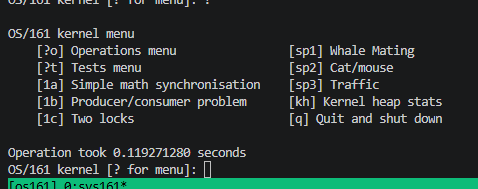
\includegraphics[width=\textwidth]{screenshots/asst1-01-debugger.png}
}{
    \fbox{
        \parbox{0.9\textwidth}{
            \centering
            Screenshot placeholder: debugger startup.
        }
    }
}
\caption{System/161 started with GDB attached}
\end{figure}

\begin{figure}[H]
\centering
\IfFileExists{screenshots/asst1-02-1a.png}{
    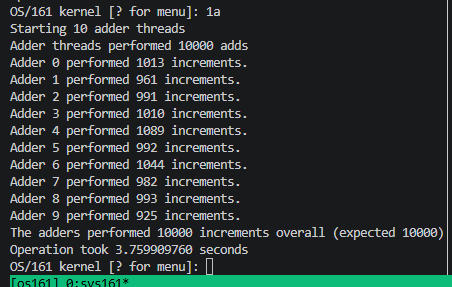
\includegraphics[width=\textwidth]{screenshots/asst1-02-1a.png}
}{
    \fbox{
        \parbox{0.9\textwidth}{
            \centering
            Screenshot placeholder: test 1a.
        }
    }
}
\caption{Successful output for 1a Concurrent Mathematics}
\end{figure}

\begin{figure}[H]
\centering
\IfFileExists{screenshots/asst1-03-1b.png}{
    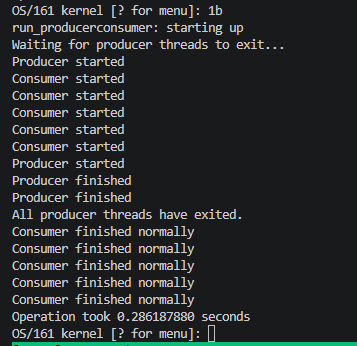
\includegraphics[width=\textwidth]{screenshots/asst1-03-1b.png}
}{
    \fbox{
        \parbox{0.9\textwidth}{
            \centering
            Screenshot placeholder: test 1b.
        }
    }
}
\caption{Successful output for 1b Producer/Consumer}
\end{figure}

\begin{figure}[H]
\centering
\IfFileExists{screenshots/asst1-04-bar.png}{
    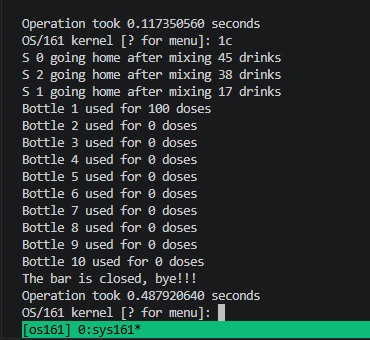
\includegraphics[width=\textwidth]{screenshots/asst1-04-bar.png}
}{
    \fbox{
        \parbox{0.9\textwidth}{
            \centering
            Screenshot placeholder: new Bar Synchronization test 1c.
            Run \texttt{1c}, capture the output, and save it as
            \texttt{screenshots/asst1-04-bar.png}.
        }
    }
}
\caption{Successful output for 1c Bar Synchronization}
\end{figure}

\section{Conclusion}

The assignment demonstrates the core synchronization problems that arise in a
kernel with concurrent threads. The math part requires mutual exclusion around
a shared counter. The producer/consumer part requires both mutual exclusion and
counting synchronization to coordinate buffer capacity. The two-locks part
requires a consistent lock acquisition order to prevent deadlock. The completed
OS/161 lock and condition-variable primitives provide the foundation required
for these solutions and for later synchronization work.

\newpage
\appendix

\section{Source Code: math.c}
\lstinputlisting[style=cstyle]{os161-1.99/kern/asst1/math.c}

\newpage
\section{Source Code: producerconsumer.c}
\lstinputlisting[style=cstyle]{os161-1.99/kern/asst1/producerconsumer.c}

\newpage
\section{Source Code: bar.c}
\lstinputlisting[style=cstyle]{os161-1.99/kern/asst1/bar.c}

\newpage
\section{Source Code: bar\_driver.c}
\lstinputlisting[style=cstyle]{os161-1.99/kern/asst1/bar_driver.c}

\newpage
\section{Source Code: synch.c}
\lstinputlisting[style=cstyle]{os161-1.99/kern/thread/synch.c}

\end{document}
